% =============================================================================
% apendiceE.tex — DESENHOS (issue 52)
% As folhas são geradas pelo pipeline (mlc_projeto/output/desenhos.py) em
% tese/fig/des*.pdf, com a largura útil da página: incluídas com \textwidth,
% a escala indicada em cada folha vale no papel.
% =============================================================================

\chapter{DESENHOS}\label{ap:desenhos}

Este apêndice reúne as folhas de desenho da estrutura, cotadas e em escala. Cada
folha tem a largura útil da página e é reproduzida em tamanho natural, de modo que
a escala indicada no rodapé vale na impressão; a escala gráfica permite conferi-la.
Os nomes dos elementos seguem a \autoref{tab:nomenclatura} e são os mesmos do
memorial. As folhas são geradas pelo programa de cálculo a partir da geometria e
dos resultados do dimensionamento, e se atualizam a cada execução.

\begin{center}
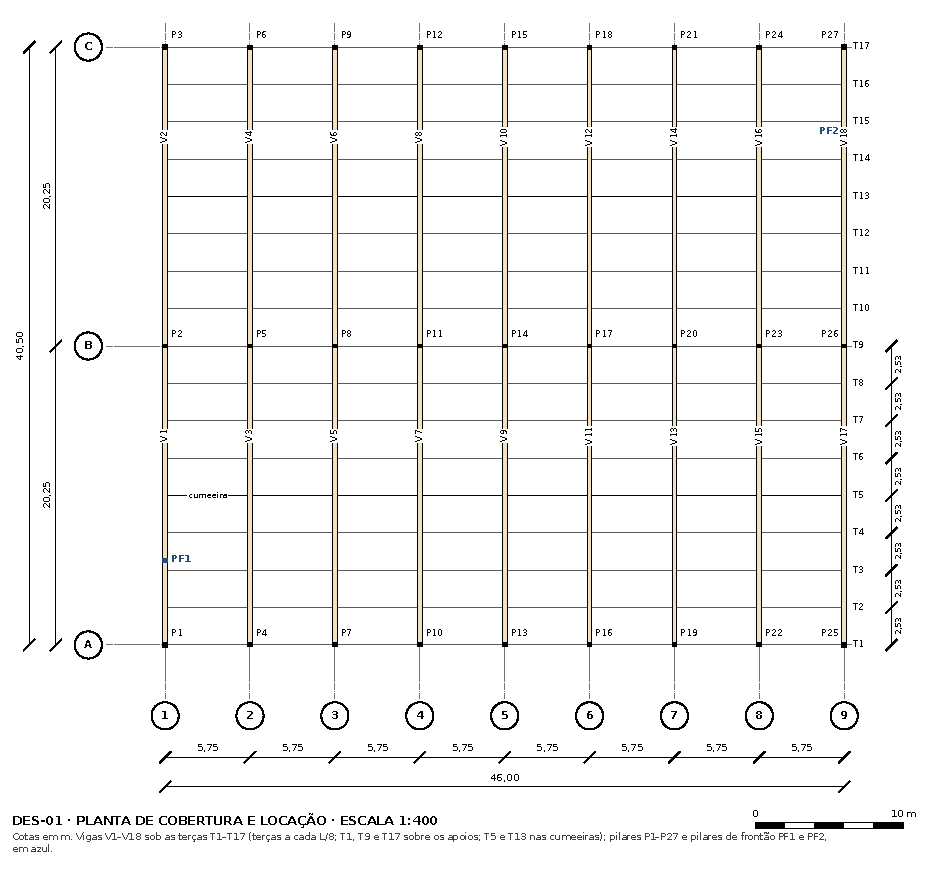
\includegraphics[width=\textwidth]{fig/des01_planta_cobertura.pdf}
\end{center}
\clearpage
\begin{center}
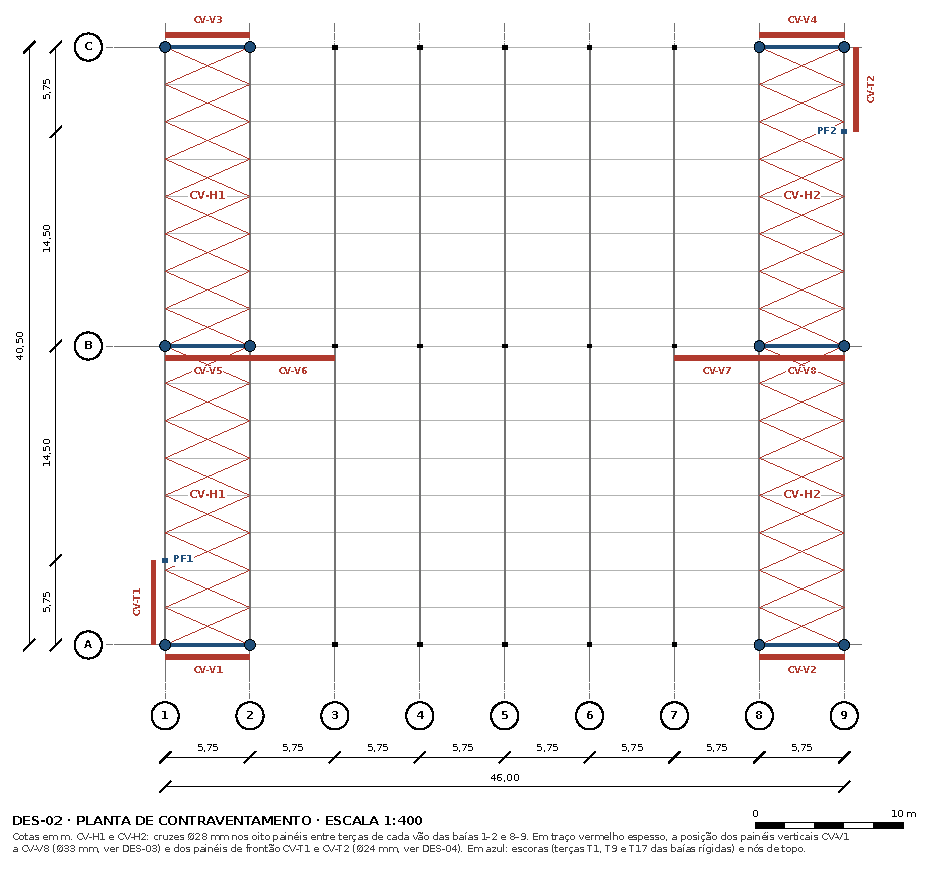
\includegraphics[width=\textwidth]{fig/des02_planta_contraventamento.pdf}
\end{center}
\clearpage
\begin{center}
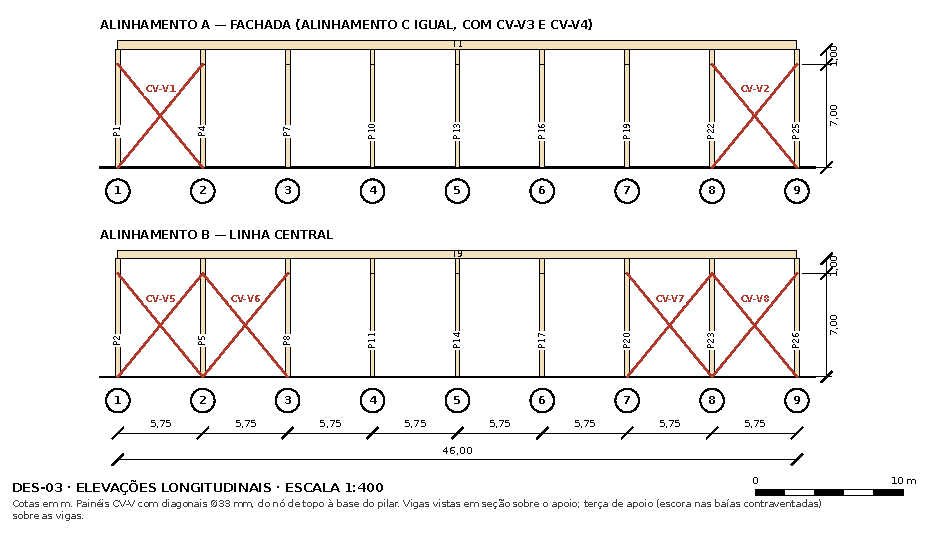
\includegraphics[width=\textwidth]{fig/des03_elevacoes_longitudinais.pdf}

\vspace{8mm}
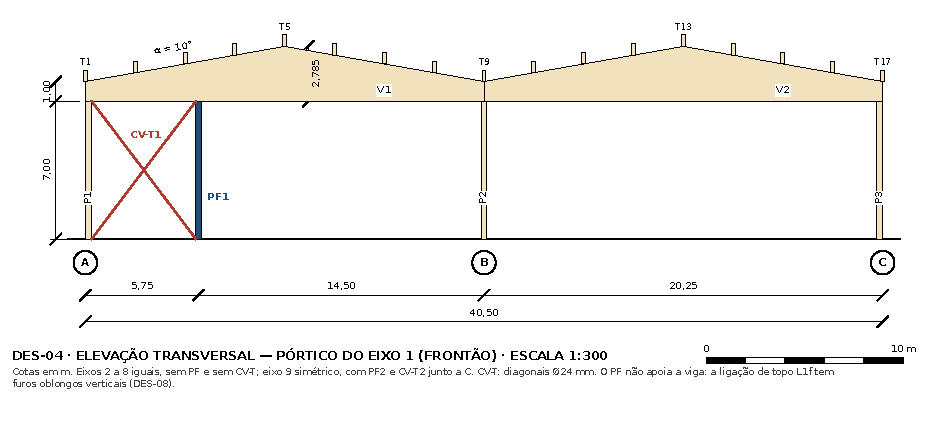
\includegraphics[width=\textwidth]{fig/des04_elevacao_transversal.pdf}
\end{center}
\clearpage
\begin{center}
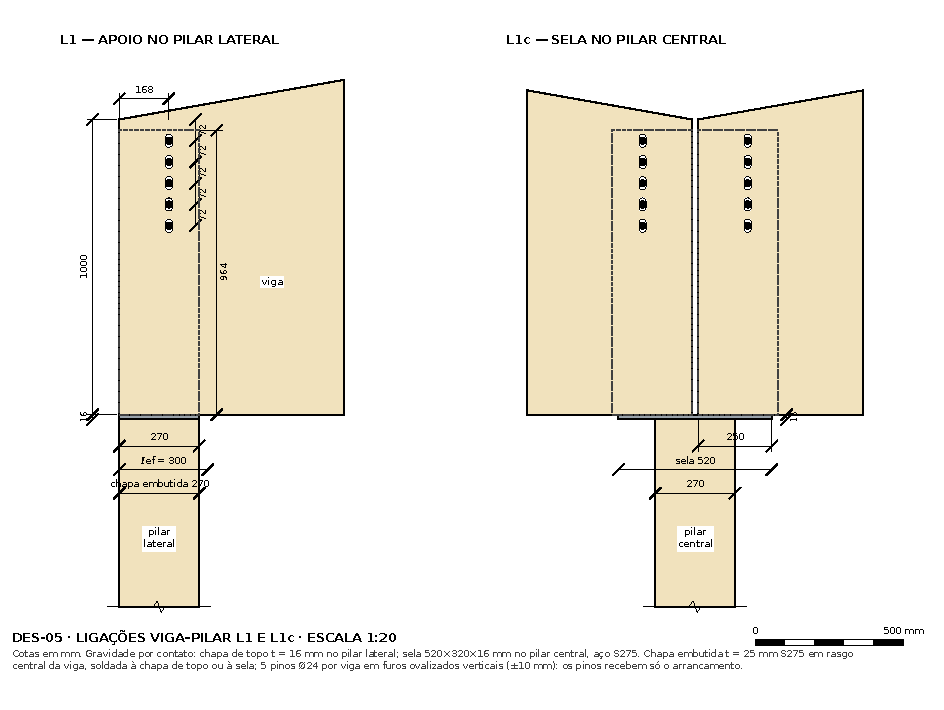
\includegraphics[width=\textwidth]{fig/des05_ligacoes_L1_L1c.pdf}

\vspace{3mm}
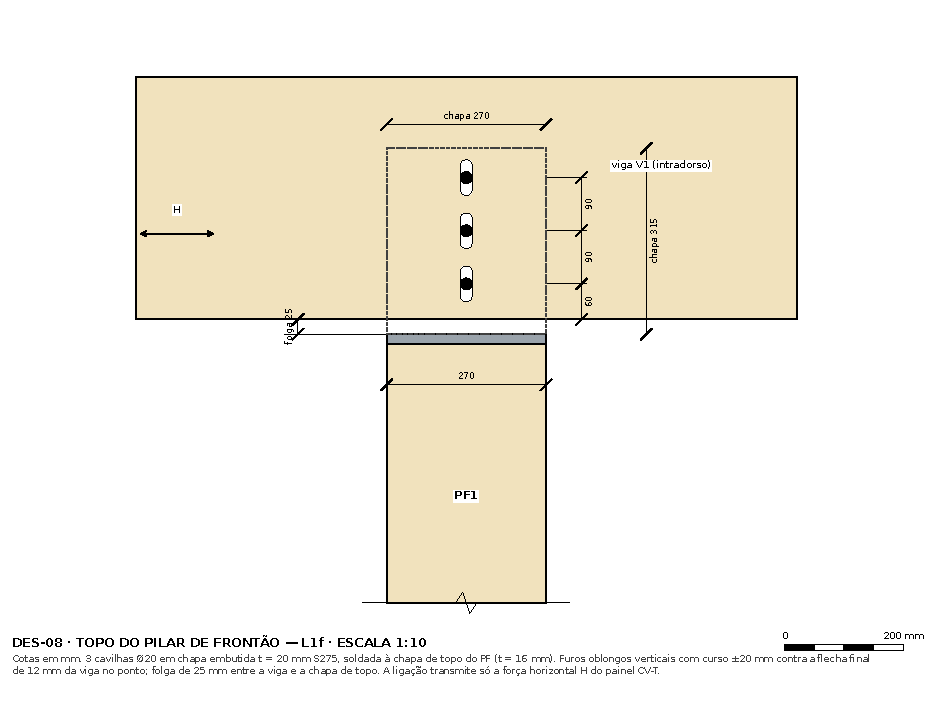
\includegraphics[width=\textwidth]{fig/des08_topo_PF_L1f.pdf}
\end{center}
\clearpage
\begin{center}
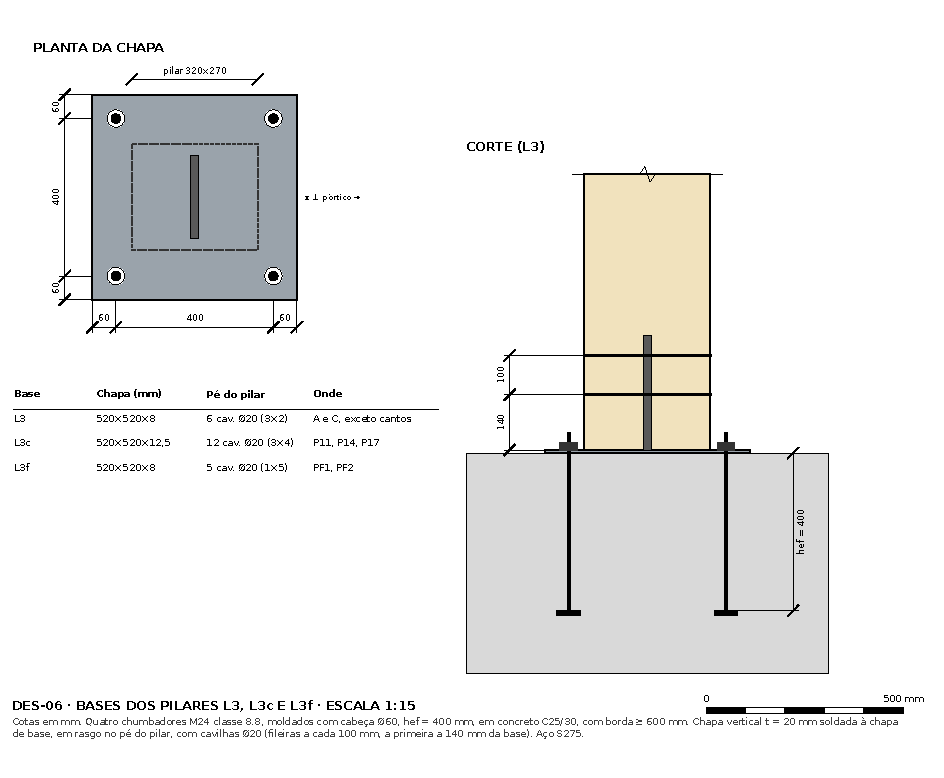
\includegraphics[width=\textwidth]{fig/des06_bases_correntes.pdf}
\end{center}
\clearpage
\begin{center}
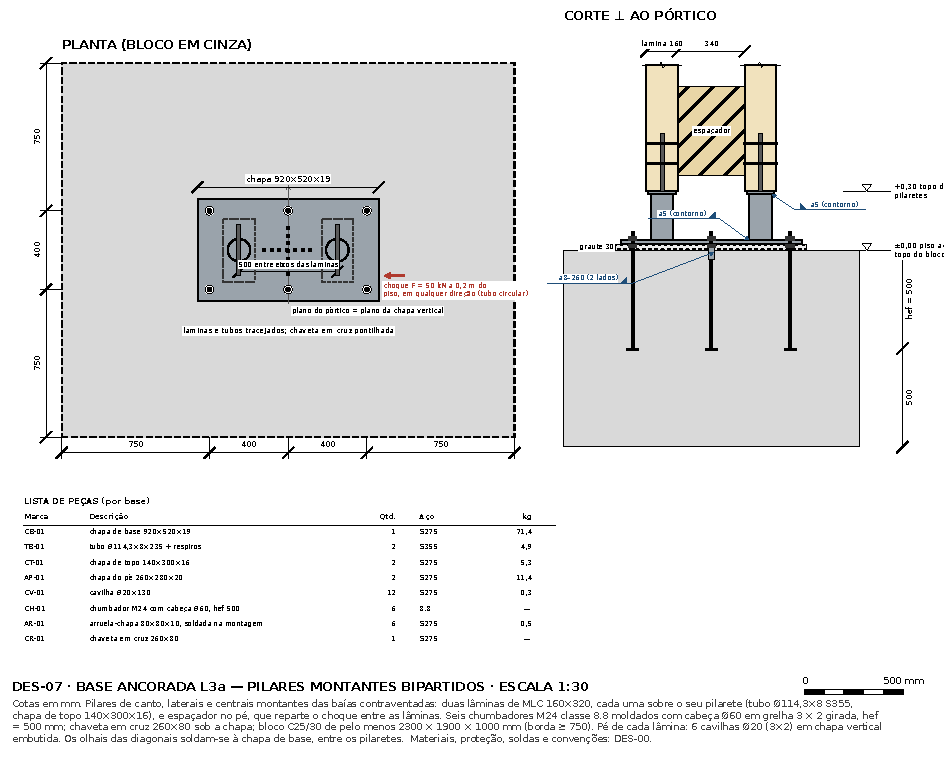
\includegraphics[width=\textwidth]{fig/des07_base_ancorada.pdf}
\end{center}
